\chapter{Search in Graphs}
\label{ch:graphsearch}

\newcommand{\lecnum}{24}
%\newcommand{\lectitle}{Search in Graphs}
\newcommand{\lecturer}{Frank Pfenning, Andr\'e Platzer, Rob Simmons,\\
  Penny Anderson, Iliano Cervesato}

\chapterTAGS{complexity, correctness, graph, traverse-ds, search}
\maketitle

\begin{preamble}
\noindent
In this lecture, we will discuss the question of \emph{graph
  reachability}: given two vertices $v$ and $w$, does there exist a
path from $v$ to $w$?
\end{preamble}

\begin{gram}[Learning Goals]
This maps as follows onto the learning goals for this course:
\begin{description}
\item[Computational Thinking: ]%
  We continue learning about graphs, and specifically about paths in a
  graph.  An important question is whether there exists a path between
  two given nodes.  A related problem is to produce this path (if it
  exists).
\item[Algorithms and Data Structures: ]%
  We explore two classic approaches to answering these questions:
  depth-first search and breadth-first search.  Both rely on the need
  to remember what we have done already, and to go back and try
  something else if we get stuck.
\item[Programming: ]%
  We give two implementations of depth-first search, one recursive
  that uses the call stack of C to remember what we have done, and the
  other iterative that uses an explicit stack for that purpose.  We
  also see that breadth-first search is the variant of the latter
  where a queue is used instead of a stack.
\end{description}
\end{gram}

\begin{gram}[graph.h]
As a reminder, we are working with the following minimal graph
interface.  We will be implementing our search in terms of this
interface.
\begin{lstlisting}[language=c]
typedef unsigned int vertex;
typedef struct graph_header *graph_t;

graph_t graph_new(unsigned int numvert);
//@ensures \result != NULL;

void graph_free(graph_t G);
//@requires G != NULL;

unsigned int graph_size(graph_t G);
//@requires G != NULL;

bool graph_hasedge(graph_t G, vertex v, vertex w);
//@requires G != NULL;
//@requires v < graph_size(G) && w < graph_size(G);

void graph_addedge(graph_t G, vertex v, vertex w);
//@requires G != NULL;
//@requires v < graph_size(G) && w < graph_size(G);
//@requires v != w && !graph_hasedge(G, v, w);

typedef struct vert_list_node vert_list;
struct vert_list_node {
  vertex vert;
  vert_list *next;
};

vert_list* graph_get_neighbors(graph_t G, vertex v);
//@requires G != NULL;
//@requires v < graph_size(G);

void graph_free_neighbors(vert_list* neighbors);
\end{lstlisting}
\end{gram}

\section{Paths in Graphs}
\label{sec:graphsearch:paths}
\TAGS{graph}

A \emph{path} in a graph is a sequence of vertices where each vertex
is connected to the next by an edge.  That is, a path is a sequence
$$
v_0, v_1, v_2, v_3, \dots, v_l
$$
of some length $l\geq0$ such that there is an edge from $v_i$ to
$v_{i+1}$ in the graph for each $i<l$.
\begin{center}
  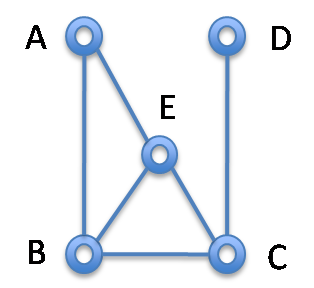
\includegraphics[width=0.3\textwidth]{img/graph0.png}
\end{center}
For example, all of the following are paths in the graph above:
$$
\begin{array}{l}
A-B-E-C-D \\
A-B-A \\
E-C-D-C-B \\
B
\end{array}
$$
The last one is a special case: The length of a path is given by the
number of edges in it, so a node by itself is a path of length 0
(without following any edges).  Paths always have a starting vertex
and an ending vertex, which coincide in a path of length 0.  We also
say that a path connects its endpoints.

The \emph{graph reachability problem} is to determine if there is a
path connecting two given vertices in a graph.  If we know the graph
is connected, this problem is easy since one can reach any node from
any other node.  But we might refine our specification to request that
the algorithm return not just a boolean value (reachable or not), but
an actual path.  At that point the problem is somewhat interesting
even for connected graphs. In complexity theory it is sometimes said
that a path from vertex $v$ to vertex $w$ is a \emph{certificate} or
\emph{explicit evidence} for the fact that vertex $w$ is reachable
from another vertex $v$.  It is easy to check whether the certificate
is valid, since it is easy to check if each node in the path is
connected to the next one by an edge.  It is more difficult to produce
such a certificate.

For example, the path
$$
A-B-E-C-D
$$
is a certificate for the fact that vertex $D$ is reachable from vertex
$A$ in the above graph.  It is easy to check this certificate by
following along the path and checking whether the indicated edges are
in the graph.

In most of what follows we are not concerned with finding the path,
but only with determining whether one exists. It is not difficult to
see how to extend the algorithms we discuss to compute the path as
well.


\section{Depth-First Search}
\label{sec:graphsearch:dfs}
\TAGS{complexity, correctness, traverse-ds, search}

The first algorithm we consider for determining if one vertex is
reachable from another is called \emph{depth-first search}.

Let's try to work our way up to this algorithm.  Assume we are trying
to find a path from $u$ to $w$.  We start at $u$.  If it is equal to
$w$ we are done, because $w$ is reachable by a path of length 0.  If
not we pick an arbitrary edge leaving $u$ to get us to some node $v$.
Now we have ``reduced'' the original problem to the one of finding a
path from $v$ to $w$.

The problem here is of course that we may never arrive at $w$ even if
there is a path.  For example, say we want to find a path from $A$ to
$D$ in our earlier example graph.
\begin{center}
  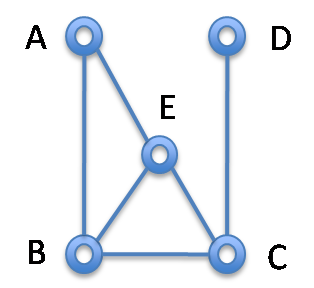
\includegraphics[width=0.3\textwidth]{img/graph0.png}
\end{center}
We can go $A-B-E-A-B-E-\cdots$ without ever reaching $D$ (or we can go
just $A-B-A-B-\cdots$), even though there exists a path.

We need to avoid repeating nodes in the path we are exploring.  A
\emph{cycle} is a path of length 1 or greater that has the same
starting and ending point.  So another way to say we need to avoid
repeating nodes is to say that we need to avoid cycles in the path.
We accomplish this by \emph{marking} the nodes we have already
considered so when we see them again we know not to consider them
again.

Let's go back to the earlier example and play through this idea while
trying to find a path from $A$ to $D$.  We start by marking $A$
(indicated by hollowing the circle) and go to $B$.  We indicate the
path we have been following by drawing a double-line along the edges
contained in it.
\begin{center}
  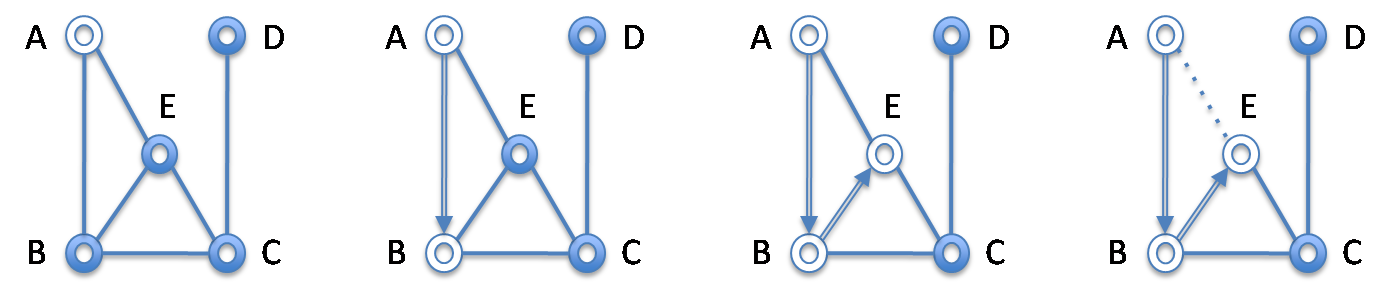
\includegraphics[width=\textwidth]{img/dfs1.png}
\end{center}
When we are at $B$ we mark $B$ and have three choices for the next
step.
\begin{enumerate}
\item%
  We could go back to $A$, but $A$ is already marked and therefore
  ruled out.
\item%
  We could go to $E$.
\item%
  We could go to $C$.
\end{enumerate}
Say we pick $E$.  At this point we have again three choices.  We might
consider $A$ as a next node on the path, but it is ruled out because
$A$ has already been marked.  We show this by dashing the edge from
$A$ to $E$ to indicate it was considered, but ineligible.  The only
possibility now is to go to $C$, because we have been at $B$ as well
(we just came from $B$).
\begin{center}
  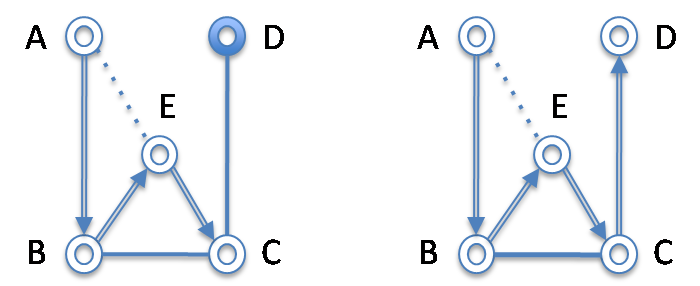
\includegraphics[width=0.5\textwidth]{img/dfs2.png}
\end{center}
From $C$ we consider the link to $D$ (before considering the link to
$B$) and we arrive at $D$, declaring success with the path
$$
A-B-E-C-D
$$
which, by construction, has no cycles.

There is one more consideration to make, namely what we do when we get
stuck.  Let's reconsider the original graph
\begin{center}
  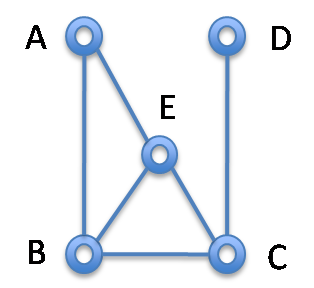
\includegraphics[width=0.3\textwidth]{img/graph0.png}
\end{center}
and the goal to find a path from $E$ to $B$.  Let's say we start $E -
C$ and then $C - D$.  At this point, all the vertices we could go to
(which is only C) have already been marked!  So we have to
\emph{backtrack} to the most recent choice point and pursue
alternatives.  In this case, this could be $C$, where the only
remaining alternative would be $B$, completing the path $E - C - B$.
Notice that when backtracking we have to go back to $C$ even though it
is already marked.

Depth-first search is characterized not only by the marking, but also
that when we get stuck we always return to our most recent choice and
follow a different path.  When no other alternatives are available, we
backtrack further.  Let's consider the following slightly larger
graph, where we explore the outgoing edges using the alphabetically
last label first. We will trace the search for a path from $A$ to $B$.
\begin{center}
  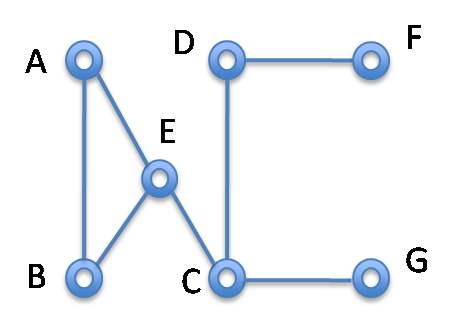
\includegraphics[width=0.4\textwidth]{img/dfs3.png}
\end{center}
We write the current node we are visiting on the left and on the right
a \emph{stack} of nodes we have to return to when we backtrack.  For
each of these we also remember which choices remain (in parentheses).
We annotate marked nodes with an asterisk, which means that we never
pick them as the next node to visit.

For example, going from step 4 to step 5 we do not consider $E^*$ but
go to $D$ instead.  We backtrack when no unmarked neighbors remain for
the current node.  We are keeping the visited nodes on a stack so we
can easily return to the most recent one. The stack elements are
separated by \lstinline'|' and the lists of neighbors are wrapped in
parentheses, e.g., $(B,A^*)$.
$$
\begin{array}{ccrll}
   \textbf{Step} & \textbf{Current}% & \text{Neighbors}
 & {\textbf{Stack}} & \textbf{Remark}
\\[1ex]
   1 & A %& (E, B)
 &
\\ 2 & E %& (C, B, A^*)
 & A^*\; (B)
\\ 3 & C %& (G, E^*, D)
 & E^*\; (B,A^*) \mid A^*\; (B)
\\ 4 & G %& (C^*)
 & C^*\; (E^*,D) \mid E^*\; (B,A^*) \mid A^*\; (B)
 & \text{Backtrack}
%\\ 5 & C^* & \text{\em don't care} & G^*\;() \mid C^*\;(E^*, D) \mid E^*\;(B, A^*) \mid A^*\;(B) & \text{Backtrack}
%\\ 6 & E^* & \text{\em don't care} & C^*\;(D) \mid E^*\;(B, A^*) \mid A^*\;(B)
\\ 5 & D %& (F, C^*)
 & C^*\;() \mid E^*\;(B, A^*) \mid A^*\;(B)
\\ 6 & F %& (D^*)
 & D^*\;(C^*) \mid C^*\;() \mid E^*\;(B, A^*) \mid A^*\;(B)
 & \text{Backtrack}
%\\ 9 & D^* & \text{\em don't care} & F^*\;() \mid D^*\;(C^*) \mid C^*\;() \mid E^*\;(B, A^*) \mid A^*\;(B) & \text{Backtrack}
%\\10 & C^* & \text{\em don't care} & D^*\;() \mid C^*\;() \mid E^*\;(B, A^*) \mid A^*\;(B) & \text{Backtrack $\times 2$}
\\ 7 & B %& (A^*)
 & E^*\;(A^*) \mid A^*\;(B)
 & \text{Goal Reached}
\end{array}
$$


\subsection{Recursive Depth-First Search}
\label{sec:graphsearch:dfs_recursive}

Now we can easily write the depth-first search code recursively,
letting the \emph{call stack} keep track of everything we need for
backtracking.

\begin{lstlisting}[language=c, numbers=left]
bool dfs_helper(graph_t G, bool *mark, vertex start, vertex target) {
  REQUIRES(G != NULL && mark != NULL);
  REQUIRES(start < graph_size(G) && target < graph_size(G));
  REQUIRES(!mark[start]);

  // mark start as seen
  mark[start] = true;

  // there is an edge from start to v and a path from v to target if...
  // target == start, or
  if (target == start) return true;
  // there is an edge from start to v ...
  vert_list *nbors = graph_get_neighbors(G, start);
  for (vert_list *p = nbors; p != NULL; p = p->next) {
    vertex v = p->vert;   // v is one of start's neighbors
    // ... and a path from v to target
    if (!mark[v] && dfs_helper(G, mark, v, target)) {
      graph_free_neighbors(nbors);
      return true;
    }
  }
  graph_free_neighbors(nbors);
  return false;
}
\end{lstlisting}
We shall free the neighbor list before each return, or risk a memory
leak.

We've named the function \lstinline'dfs_helper' because the user of the
search should not have to worry about supplying the array of
marks. Instead the user calls the function \lstinline'dfs', below, which
creates the marks and passes them to the recursive helper function.
\begin{lstlisting}[language=c, numbers=left, firstnumber=26]
bool dfs(graph_t G, vertex start, vertex target) {
  REQUIRES(G != NULL);
  REQUIRES(start < graph_size(G) && target < graph_size(G));

  bool *mark = xcalloc(graph_size(G), sizeof(bool));
  bool connected = dfs_helper(G, mark, start, target);
  free(mark);
  return connected;
}
\end{lstlisting}

What is the cost of recursive DFS for a graph with $v$ vertices and
$e$ edges?

The function \lstinline'dfs' creates an array of marks with all
positions initialized to zero (i.e., to \lstinline'false') on
line 30.  Although this array has $v$ elements, the
operating system, which ultimately appropriates the blocks of memory
handed out by \lstinline'malloc' and \lstinline'calloc', is able to
perform this operation in about $O(1)$ time.  The call to
\lstinline'free' is also constant time.  Therefore, the asymptotic
complexity of \lstinline'dfs' is equal to the cost of the call to
\lstinline'dfs_helper' on line 31.

The analysis of \lstinline'dfs_helper' bears similarities to that of
\lstinline'graph_print' in the last chapter, with the novelty that
\lstinline'dfs_helper' is recursive rather than iterative.  The call
to \lstinline'graph_get_neighbors' on line 13 has
constant cost in the adjacency list representation and costs $O(v)$ in
the adjacency matrix representation.  The body of the loop on
lines 14--21 runs $O(e)$ times
\emph{overall} since every edge will be visited exactly twice
altogether (once from each direction).  In particular,
line 15 is run $O(e)$ times altogether.

This entails that there will be at most $2e$ recursive calls to
\lstinline'dfs_helper'.  Furthermore, lines 4 and 7,
and the fact that marks are never reset,
ensures that this function will be called no more than $v$ times.
Thus, there can be at most $\min(2e, v)$ recursive calls to
\lstinline'dfs_helper'.

Each call to \lstinline'graph_free_neighbors' costs $O(1)$ in the
adjacency list representation while they altogether cost $O(e)$ in the
adjacency matrix representation.  All other operations in
\lstinline'dfs_helper' have constant cost, and therefore
$O(\min(e,v))$ overall since there are at most $\min(2e,v)$ recursive
calls.

Tallying up all these components, we have an $O(e)$ worst case
complexity for the call to \lstinline'dfs_helper' on
line 31 with an adjacency list representation and
$O(\min(v^2,ev))$ for the adjacency matrix representation --- the
latter is often simplified to $O(v^2)$ since most graphs encountered
in realistic applications have at least $O(v)$ edges.  This is also
the cost of \lstinline'dfs'.


\subsection{Depth-First Search with an explicit stack}
\label{sec:graphsearch:dfs_iterative}

When scrutinizing the above example, we notice that the sophisticated
data structure of a stack of nodes with their adjacency lists was
really quite unnecessary for DFS.  The recursive implementation is
simple and elegant, but its effect is to make the data management more
complex than necessary: all we really need for backtracking is a stack
of nodes that have been seen but not yet considered.

This can all be simplified by making the stack explicit. In that case
there is a single stack with all the nodes on it that we still need to
look at. (In the sample code in Figure~\ref{fig:dfs-explicit}, we use
a stack specialized to hold things of type \lstinline'vertex' just to
keep the code simple.)

\medskip
\begin{tabular}{rllr}
   {\bf Step} & {\bf Current} & {\bf Neighbors}
 & {\bf New stack}
\\ 0 &  &  & $(A^*)$
\\ 1 & $A^*$ & $(E,B)$       & $(E^*,B^*)$
\\ 2 & $E^*$ & $(C,B^*,A^*)$ & $(C^*,B^*)$
\\ 3 & $C^*$ & $(G,E^*,D)$   & $(G^*,D^*,B^*)$
\\ 4 & $G^*$ & $(C^*)$       & $(D^*,B^*)$
\\ 5 & $D^*$ & $(F, C^*)$    & $(F^*, B^*)$
\\ 6 & $F^*$ & $(D^*)$       & $(B^*)$
\\ 7 & $B^*$ & $(E^*,A^*)$   & $()$
\end{tabular}
\medskip

\begin{gram}[DFS With an Explicit Stack]
\label{fig:dfs-explicit}
\begin{lstlisting}[language=c, numbers=left]
bool dfs_explicit_stack(graph_t G, vertex start, vertex target) {
  REQUIRES(G != NULL);
  REQUIRES(start < graph_size(G) && target < graph_size(G));

  if (start == target) return true;

  // mark is an array containing only the start
  bool *mark = xcalloc(graph_size(G), sizeof(bool));
  mark[start] = true;

  // Work list initially containing only start
  istack_t S = stack_new();
  push(S, start);

  while (!stack_empty(S)) {
  // Loop invariants to prove correctness go here
    vertex v = pop(S);      // v is the current node
    vert_list *nbors = graph_get_neighbors(G, v);
    for (vert_list *p = nbors; p != NULL; p = p->next) {
      vertex w = p->vert;  // w is one of v's neighbors
      if (w == target) {   // if w is the target return true
        graph_free_neighbors(nbors);
        stack_free(S);
        free(mark);
        return true;       // Success!
      }
      if (!mark[w]) {      // if w was not seen before
        mark[w] = true;       // Mark it as known
        push(S, w);           // Add to work list
      }
    }
    graph_free_neighbors(nbors);
  }
  stack_free(S);
  free(mark);
  return false;
}
\end{lstlisting}
\end{gram}


In the code in Figure~\ref{fig:dfs-explicit}, we mark the starting
node and push it on the stack.  Then we iteratively pop the stack and
examine each neighbor of the node we popped. If the neighbor is not
already marked, we push it on the stack to make sure we look at it
eventually. If the stack is empty then we've explored all
possibilities without finding the target, so we return
\lstinline'false'.

\medskip

While convincing, this explanation comes short of a proof that our
implementation is correct, i.e., that it returns \lstinline'true' when
there is a path between \lstinline'start' and \lstinline'target' and
returns \lstinline'false' otherwise.  We will now develop a more solid
argument, although we will stop short of a formal proof.  The function
\lstinline'dfs_explict_stack' returns in exactly three places.  The
first is on line 5, when \lstinline'start' is equal to
\lstinline'target'.  By definition, there is a degenerate path between
these two nodes in this case.

The other two places where the function returns,
lines 25 and 36, have us go through loops.
To reason about loops, we need to develop loop invariants that we will
squeeze in the placeholder on line 16.  We start with the
return statement on line 25: we know that \lstinline'w'
(which is equal to \lstinline'target' by line 21) is a
neighbor of vertex \lstinline'v', but how do we know that there is a
path from \lstinline'start' to \lstinline'v'?  Two invariants will
prove helpful here:
\begin{enumerate}\em
\item%
  Every marked vertex (i.e., a vertex \lstinline'u' such that
  \lstinline'mark[u] == true') is connected to \lstinline'start'.
\item%
  Every vertex in the stack is marked.
\end{enumerate}
These two invariants hold initially since \lstinline'start' is the
only marked vertex and the only item in the stack before the loop is
run the first time.  They are preserved by an arbitrary iteration of
the loop since only neighbors of \lstinline'v' (which is assumed to be
reachable from \lstinline'start') are marked on line 28
and they are immediately pushed on the stack on line 29.
Therefore, if the loop exits at line 25, we know that
there is a path from \lstinline'start' to \lstinline'target'.

These two invariants are not sufficient to prove that there is no path
from \lstinline'start' to \lstinline'target' if the function returns
\lstinline'false' on line 36.  For this, we need a new
concept and a new invariant involving it.  The new concept is that of
\emph{frontier} of the search.  The frontier is a set of vertices that
we know are connected to \lstinline'start' but that we have not
explored yet.  At any point in the loop on
lines 15--33, the frontier is the
contents of the stack.  The new invariant is the following:
\begin{enumerate}\em
\item[3]%
  Every path from \lstinline'start' to \lstinline'target' passes
  through a vertex in the frontier.
\end{enumerate}
It is clearly true initially when the stack (the frontier) only
contains \lstinline'start'.  It is preserved by the loop because
intuitively a frontier element is replaced by all of its neighbors
that have not been explored already.  More interesting is why this
invariant allows us to prove that there is no path to
\lstinline'target' if the function returns on line 36:
for this to happen, we must have exited the loop in
lines 15--33, which entails that the
negation of its loop guard is true: the stack (our frontier) is empty.
By our third invariant (which still holds at this point), every path
from \lstinline'start' to \lstinline'target' must go through a vertex
in the frontier.  But the frontier is empty, so it contains no vertex
through which such a pass can go: thus, there cannot be any path from
\lstinline'start' to \lstinline'target'.  Only in this way can the
invariant be true, if the frontier is empty: if all of zero paths from
\lstinline'start' to \lstinline'target' pass through one of the (zero)
vertices in the empty frontier.

\medskip

The complexity considerations we developed for the recursive version
of DFS apply here as well --- possibly more explicitly.  The above
code has cost $O(e)$ with an adjacency list representation:
initializing the array of marks has cost $O(1)$, and the body of the
inner loop will run $O(e)$ times, twice for each edge.  The cost is
$O(\min(v^2,ev))$ --- just $O(v^2)$ in most situations --- with an
adjacency matrix representation as we have to account for the $O(v)$
cost of \lstinline'graph_get_neighbors'.


\section{Breadth-First Search}
\label{sec:graphsearch:bfs}
\TAGS{traverse-ds, search}

The iterative DFS algorithm managed its agenda, i.e., the list of
nodes it still had to look at, using a stack.  But there's no reason
to insist on a stack for that purpose.  What happens if we replace the
stack by a queue?  All of a sudden, we will no longer explore the most
recently found neighbor first as in depth-first search, but, instead,
we will look at the oldest neighbor first.  This corresponds to a
\emph{breadth-first search} (BFS) where you explore the graph layer by
layer.  So BFS completes a layer of the graph before proceeding to the
next layer.  The code for that and many other interesting variations
of graph search can be found on the course web page.

Here's an illustration using our running example of search for a path
from $A$ to $B$ in the graph
\begin{center}
  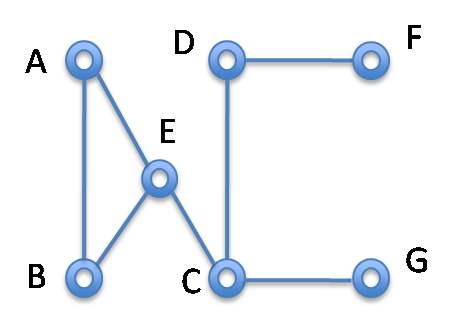
\includegraphics[width=0.4\textwidth]{img/dfs3.png}
\end{center}

\medskip
\begin{tabular}{rlll}
  Step & Current & Neighbors & New queue \\
  0 &  &  & $(A^*)$ \\
  1 & $A^*$ & $(E,B)$ & $(E^*,B^*)$ \\
  2 & $E^*$ & $(B^*, A^*, C)$ & $(B^*, C^*)$ \\
  3 & $B^*$ & $(E^*,A^*)$ & $(C^*)$ \\
\end{tabular}

\medskip
We find the path much faster this way. But this is just one
example. Try to think of another search in the same graph that would
cause breadth-first search to examine more nodes than depth-first
search would.

The code looks the same as our iterative depth-first search, except
for the use of a queue instead of a stack. Therefore we do not include
it here. You could write it yourself, and if you have difficulty, you
can find it in the code folder that goes with this lecture.  Note that
our correctness and complexity analysis for DFS never relied on using
a stack.  Thus, it remains sound once we swap the stack for a queue.
Correctness also hold for any other implementation of work list, but
complexity may need to be revisited if these implementation cannot
provide constant-time insertion and retrieval operations.


\section{Conclusion}
\label{sec:graphsearch:conclusion}
\TAGS{traverse-ds}

Breadth-first and depth-first search are the basis for many
interesting algorithms as well as search techniques for artificial
intelligence.

One potentially important observation about breadth-first versus
depth-first search concerns search when the graph remains implicit,
for instance in game search. In this case there might be infinite
paths in the graph.  Once embarked on such a path depth-first search
will never backtrack, but will pursue the path
endlessly. Breadth-first search, on the other hand, since it searches
layer by layer, is not subject to this weakness (every node in a graph
is limited to a finite number of neighbors). In order to get some
benefits of both techniques, a technique called \emph{iterative
  deepening} is sometimes used.


% \clearpage
% \section*{Exercises}

% \clearpage
% \bibliographystyle{alpha}
% \bibliography{modal}
